\section{GeoGate: The Tested Late Schedule}
\label{sec:method}
GeoGate combines late-prefill pruning with all-layer prompt-cache compaction before decoding (\cref{fig:method}). Reported quality and cost concern this joint intervention. \emph{L14 pruning} runs zero-indexed block L14 at full length, then prunes its output before L15. The default retains $R=0.10$ of spatial tokens; separate fixed-budget comparisons use $K=128$ and are distinct from R10. The schedule changes neither weights nor training data.

\begin{figure*}[t]
\centering
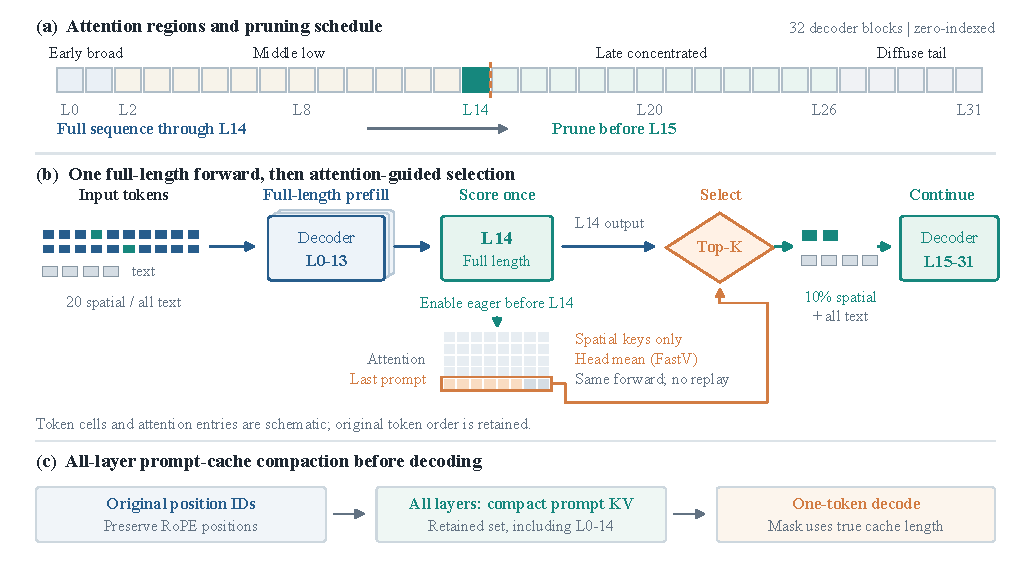
\includegraphics[width=\textwidth]{fig2_geogate_method.pdf}
\caption{\textbf{GeoGate execution.} We enable eager attention before running L14 at full length. FastV's head-averaged last-prompt score from that forward pass selects spatial tokens before L15. All text tokens and original rotary position embedding (RoPE) position IDs remain. The tested decode interface compacts every layer's prompt KV cache, including earlier layers, to the final retained set and feeds one token per step.}
\label{fig:method}
\end{figure*}

\textbf{Scoring and execution.} Let $\mathbf{A}$ denote head-averaged attention from the full-length pruning-block forward pass, and let $T$ be the total prompt length. For spatial span $[s_0,s_1)$ and last prompt position $g=T-1$:
\begin{align}
s_i &= \mathbf{A}_{g,\,i},\quad i\in[s_0,s_1),\\
\mathcal{I}_{\text{top}} &= \operatorname*{top\text{-}K}_{i\in[s_0,s_1)}(s_i),
\end{align}
where $K=\max(1,\operatorname{round}(R\,N_{\text{spatial}}))$ uses nearest-integer ties-to-even rounding and is capped at $N_{\text{spatial}}$, the number of spatial tokens. The kept set contains all non-spatial tokens and the selected spatial tokens:
\begin{equation}
\mathcal{I}_{\text{kept}} \;=\; [0,s_0)\;\cup\;\mathcal{I}_{\text{top}}\;\cup\;[s_1,T).
\end{equation}
We apply the kept indices in ascending original-position order and preserve each retained token's original rotary position embedding (RoPE) position ID.

\begin{center}
\small
\fbox{\begin{tabular}{@{}p{0.92\columnwidth}@{}}
\textbf{Algorithm 1: One-pass GeoGate prefill}\\
\hline
\textbf{Input:} token sequence, spatial span, $L_p=14$, $R=0.10$.\\
\textbf{1. Prepare.} Set block $L_p$ to eager attention \emph{before}
its forward; initialize the original-position map.\\
\textbf{2. Forward and score.} Run blocks $0..L_p$ once at full length.
Read the last-prompt row from that same $L_p$ forward; choose top-$K$
spatial entries and preserve all text entries.\\
\textbf{3. Reduce.} Slice hidden states, mask, and the map to the kept
set. Preserve original RoPE position IDs.\\
\textbf{4. Finish prefill.} Run blocks $L_p+1..L-1$ on the reduced
sequence. No scorer replay or second $L_p$ forward is required.\\
\textbf{5. Prepare decode.} Map each layer's KV cache to the final
original-position set; rebuild the common mask and feed one token per
decode step.\\
\end{tabular}}
\end{center}

The common-mask decode interface requires synchronized caches, including those from full-length blocks. The experiments therefore do not isolate cache compaction from prefill pruning. Generation timing includes eager attention, selection, and cache indexing; the supplement specifies the index map, deterministic scene cap, and failure diagnostics.

\textbf{Analytical cost.} Let $d=4096$ denote hidden width, $I=11008$ feed-forward width, and $L=32$ the number of decoder blocks. The total prompt lengths before and after pruning are $T$ and $T_{\text{kept}}$, including text. We model per-layer prefill cost as $f(s)=as+bs^2$, with $a=4d^2+3dI$, $b=2d$, and $q=(L_p+1)/L$:
\begin{equation}
\frac{\Phi_{\text{GeoGate}}}{\Phi_{\text{base}}}
=q+(1-q)\frac{f(T_{\text{kept}})}{f(T)}
\approx 0.577.
\end{equation}
For $T=1717$ and $T_{\text{kept}}=370$, prefill comprises 15 full-length blocks and 17 reduced blocks. Assuming eight decode steps gives a total LM ratio of 0.579, or 42.1\% fewer LM FLOPs. All-layer compaction gives a prompt-cache ratio of $T_{\text{kept}}/T=0.2155$, corresponding to 78.5\% lower storage. This storage estimate uses prompt-initialization lengths and excludes growth from generated tokens. Across one-to-32-step assumptions, the FLOP reduction ranges from 41.6--42.2\%. These analytical estimates exclude the visual encoder, selection, and cache indexing; total GPU memory and latency therefore require separate measurements.
